%% LyX 2.2.0 created this file.  For more info, see http://www.lyx.org/.
%% Do not edit unless you really know what you are doing.
\documentclass[12pt,oneside,bahasa]{book}
\usepackage{charter}
\usepackage[T1]{fontenc}
\usepackage[latin9]{inputenc}
\usepackage[letterpaper]{geometry}
\geometry{verbose,tmargin=3cm,bmargin=3cm,lmargin=4cm,rmargin=3cm}
\usepackage{fancyhdr}
\pagestyle{fancy}
\setcounter{secnumdepth}{5}
\setcounter{tocdepth}{5}
\usepackage{array}
\usepackage{float}
\usepackage{graphicx}
\usepackage{setspace}
\onehalfspacing

\makeatletter

%%%%%%%%%%%%%%%%%%%%%%%%%%%%%% LyX specific LaTeX commands.
%% Because html converters don't know tabularnewline
\providecommand{\tabularnewline}{\\}

%%%%%%%%%%%%%%%%%%%%%%%%%%%%%% User specified LaTeX commands.
%% \renewcommand{\chapter}[1]{\chapter[#1]{\centering #1}}
\usepackage{titlesec}
\usepackage{graphicx}
\titleformat{\chapter}[display]
  {\normalfont\huge\bfseries\centering}{\chaptertitlename\ \thechapter}{20pt}{\Huge}
\newcommand{\Judul}{Beternak bebek dengan menggunakan metoda Agile dan pendekatan Usability}
\newcommand{\JudulInggris}{Duck development using Agile and Usability approach}
\newcommand{\Penulis}{Jagoan Neon}
\newcommand{\NPM}{01234567}
\newcommand{\NIRM}{98432324243}
\newcommand{\JenisTulisan}{Penulisan Ilmiah}
\newcommand{\Gelar}{Jenjang DIII / Setara Sarjana Muda}
\newcommand{\Jurusan}{Sistem Informasi}
\newcommand{\Prodi}{Direktorat Program Diploma Tiga Teknologi Informasi}
\newcommand{\Tahun}{2020}
\newcommand{\Bulan}{November}
\newcommand{\Tanggal}{24}
\newcommand{\Kota}{Jakarta}
\newcommand{\KataKunci}{Teori antrian, model antrian, (FIFO/$\sim$/$\sim$)}
\newcommand{\KeyWords}{Queuing theory, queieing model}
\newcommand{\KoordinatorPI}{Dr. Batman Suratman}
\newcommand{\KetuaJurusan}{Gugum Gumbira PhD}
\newcommand{\Pembimbing}{Prof. Dr. Gundala Putra Petir, SSi, MSc}
\newcommand{\Ringkasan}{Tulis ringkasan skripsi, pi, atau apa dengan bahasa yang jelas, lugas dan
menggambarkan secara singkat tulisan ini.  Sebaiknya tidak lebih dari 150 kata
dan sudah menjelaskan dari permasalahan, pembahasan dan penutup.}
\newcommand{\JumlahPustaka}{8}
\newcommand{\JumlahHalaman}{80}
\newcommand{\JumlahHalamanDepan}{10}
\newcommand{\TahunPustaka}{1980-1993}
%%
%% Keterangan administratif sidang sarjana
%%
\newcommand{\TanggalSidang}{14 Februari 1998}
\newcommand{\TanggalLulus}{14 Februari 1998}
\newcommand{\TanggalSah}{6 April 1998}
\newcommand{\PejabatBagianSidang}{Drs. Edi Sukirman, MM}
\setlength{\headheight}{15pt}

\pagestyle{fancy}
\renewcommand{\chaptermark}[1]{\markboth{Chapter  \thechapter.\ #1}{}}
\renewcommand{\sectionmark}[1]{\markright{\thesection.\ #1}{}}

\fancyhf{}
\fancyhead[LE,RO]{\thepage}
\fancyhead[RE]{\textit{\nouppercase{\leftmark}}}
\fancyhead[LO]{\textit{\nouppercase{\rightmark}}}

\fancypagestyle{plain}{ %
\fancyhf{} % remove everything
\fancyfoot[C]{\thepage}
\renewcommand{\headrulewidth}{0pt} % remove lines as well
\renewcommand{\footrulewidth}{0pt}}

\makeatother

\usepackage{babel}
\begin{document}
\hyphenation {meng-hi-lang-kan pa-ling li-sen-si ge-ne-ral di-tam-bah
             me-nge-nai da-pat kom-pu-ter ke-dua di-ban-ding-kan
             de-ngan sa-dar meng-aki-bat-kan ber-da-sar-kan
             ke-ti-dak-ha-ti-ha-ti-an me-la-ku-kan di-be-ri-kan
             mem-ba-tasi pe-ne-kan-an ber-ka-it-an me-nya-lin
             me-nye-bar-lu-as-kan ber-asal men-dis-tri-bu-si-kan
             ma-na-kah meng-ha-sil-kan peng-ubah-an awal di-be-ri-kan
             meng-hor-mati mi-sal-nya mi-sal pu-blik pro-ses 
             meng-atur ke-cen-de-rung-an di-ra-ha-sia-kan 
             pa-ten pe-ne-ri-ma hu-kum di-nya-ta-kan wa-lau-pun
             mes-ki-pun di-se-rah-kan un-dang-un-dang ada-nya
             per-lin-dung-an meng-u-bah mem-pu-nyai ter-da-pat
             pe-mro-gram-an ini-lah ke-ta-kut-an men-da-pat-kan
             re-pu-blik in-do-ne-sia pe-ngem-bang-an ke-nya-ta-an 
             pan-dang-an di-ka-te-go-ri-kan ke-sim-pul-an 
             ka-lang-an se-pan-jang pe-ner-je-mah-an ingin-kan
             di-im-ple-men-ta-si-kan pen-ting ke-ingin-an
             meng-emu-la-si de-fi-ni-si-kan sam-ping apli-ka-si
             me-nyim-pan ma-na-ger kon-fi-gu-ra-si user ha-lam-an
             per-mo-hon-an sa-ngat suatu ma-nu-al me-na-ngani 
             di-li-hat du-kung-an ter-je-mah-an-nya ter-je-mah-an 
             ling-kung-an di-sim-pan meng-u-sa-ha-kan sa-ngat-lah
             me-re-pre-sen-ta-si-kan pe-nyim-pan-an se-ring
             spa-nyol me-nying-kat-nya apli-ka-si-nya
             ke-nya-ta-an-nya me-nge-lu-ar-kan desk-top in-ter-face
             in-ter-net ke-ku-rang-an me-mung-kin-kan fol-der 
             me-nye-ret-nya meng-u-bah-nya me-ngor-ban-kan
             peng-a-tur-an pe-nam-pil-an di-ki-rim-kan 
             meng-en-krip-si-nya pi-lih per-so-nal-iza-ti-on 
             pre-fer-en-si meng-kon-fi-gu-ra-si-kan-nya di-tam-pil-kan
             lam-pir-an be-be-ra-pa meng-a-cu pe-ngi-rim peng-a-tur-an 
             chall-enge meng-o-ten-ti-fi-ka-si me-nyim-pan-nya 
	     me-nye-dia-kan di-kem-bang-kan meng-u-bah pe-rang-kat 
	     send-mail di-gu-na-kan plat-form mem-for-mat ko-or-di-na-tor 
	     meng-gu-na-kan me-ngua-sai mem-bu-tuh-kan root line 
	     di-se-suai-kan me-ngi-rim-kan ope-ra-si se-ring-ka-li 
             di-gi-tal mem-ban-ding-kan meng-a-na-li-sa fe-no-me-na 
             peng-o-lah-an usa-ha pe-mi-lih-an fa-si-li-tas me-mo-ri 
             ke-hi-dup-an di-man-fa-at-kan me-la-in-kan bia-sa-nya 
             meng-hu-bung-kan se-tiap un-tuk olah-ra-ga standard
             men-de-fi-ni-si-kan mo-ni-toring ke-ter-se-dia-an
             de-ngan ke-sim-pul-an bia-sa-nya be-be-ra-pa peng-am-bil-an 
             peng-alam-an or-ga-ni-sa-si or-ga-ni-sa-si-nya meng-ikuti ingin-kan
             me-me-cah-kan pri-ba-di}
 
\sloppy 
\thispagestyle{empty}

\title{Membuat Aplikasi Sistem Antrian Pendaftaran Rumah Sakit}

\author{Ivans Ardiansyah}

\maketitle
\newpage{}

\thispagestyle{empty}

\pagenumbering{roman}

\vspace*{10mm}

\begin{center}
\textbf{\huge{}UNIVERSITAS GUNADARMA}
\par\end{center}{\huge \par}

\begin{center}
\textbf{FAKULTAS ILMU KOMPUTER \& TEKNOLOGI INFORMASI}
\par\end{center}

\vspace*{12mm}

\begin{center}

\includegraphics[width=35mm]{Gambar/LogoGunadarma}
\par\end{center}

\vspace*{6mm}

\begin{center}
\textbf{\Large{}PENULISAN ILMIAH}
\par\end{center}{\Large \par}

\vspace*{1cm}

\noindent \begin{center}
\begin{tabular}{|>{\centering}m{13cm}|}
\hline 
\centering{}~~\tabularnewline
\centering{}Membuat Aplikasi Sistem Antrian Pendaftaran Rumah Sakit\tabularnewline
~~\tabularnewline
\centering{}%
\begin{tabular}{lcl}
Nama & : & Ivans Ardiansyah\tabularnewline
NPM & : & 14113585\tabularnewline
Program Studi & : & Sistem Informasi\tabularnewline
Pembimbing & : & \tabularnewline
\end{tabular}\tabularnewline
~~\tabularnewline
\hline 
\end{tabular}
\par\end{center}

 \vspace*{10mm}

\begin{center}
{\large{}Diajukan Guna Memperoleh Gelar Setara Sarjana Muda}\vspace{3mm}
\par\end{center}

\begin{center}
{\large{}Universitas Gunadarma}
\par\end{center}{\large \par}

\begin{center}
{\large{}\vspace*{3mm}
2016}
\par\end{center}{\large \par}

\tableofcontents{}

\listoffigures

\listoftables


\chapter{Pendahuluan}

\setcounter{page}{1}
\pagenumbering{arabic}

\section{Latar Belakang}

Antrian merupakan kejadian yang dapat kita ditemui di berbagai tempat
yang memberikan pelayanan kepada masyarakat diantaranya rumah sakit,
bank, jalan tol dan lainya. Proses mengantri merupakan hal yang membosankan
bagi masyarakat kita karena berbagai hal, antara lain proses mengatri
yang panjang, ruang tempat menunggu antrian kurang nyaman dan sistem
antrian yang kurang bisa memberikan pengaturan antrian terhadap masyarakat.

Dengan menggunakan sistem antrian berbasis software, pengguna akan
dimudahkan dalam melakukan penambahan dokter, pengaturan kuota antrian
serta penambahan jumlah konter. 

Berangkat dari masalah itulah penulis mencoba untuk membuat sebuah
aplikasi web yang didalamnya dapat mempercepat dan mempermudah suatu
instansi rumah sakit dalam melayani masyarakat dalam pengaturan antrian. 

\section{Batasan Masalah}
\begin{enumerate}
\item Kerja aplikasi meliputi membuat, mencetak dan memanggil nomor antrian
dengan panggilan suara. 
\item Pengembangan modul pemanggilan suara menggunakan panggilan dalam Bahasa
Indonesia dengan menggunakan satu model suara perempuan. 
\end{enumerate}

\section{Tujuan Penulisan}

Tujuan dari penulisan ilmiah ini adalah untuk membuat sebuah aplikasi
web mengenai sistem pengaturan dan pemanggilan nomor antrian yang
dapat di terapkan dalam membantu suatu instansi rumah sakit dalam
mengatur proses pendaftaran masyarakat.

\section{Metode Penulisan }

Metode yang digunakan penulis dalam mengumpulkan data.
\begin{enumerate}
\item Riset Kepustakaan ( \textit{Library Research} )

Penulis melakukan riset kepustakaan dengan membaca literatur-literatur
yang berhubungan dengan objek penulisan ditambah dengan bahan kuliah
serta sumber-sumber lain yang mendukung penulisan ini.
\item Riset Lapangan ( \textit{Field Research} )

Usaha yang dilakukan oleh penulis untuk memperoleh data adalah dengan
kunjungan langsung ke sebuah rumah sakit serta mendapat informasi
dari IT rumah sakit tersebut.
\end{enumerate}

\section{Sistematika Penulisan}

Dalam penulisan ilmiah ini penulis membaginya kedalam empat bab, yaitu
sebagai berikut :
\begin{itemize}
\item BAB I PENDAHULUAN

Dalam bab ini penulis akan menguraikan dan menjelaskan latar belakang
masalah yang dihadapi, pembatasan masalah, tujuan penulisan, metode
penulisan dan sistematika penulisan yang digunakan untuk menyelesaikan
permasalahan yang ada.
\item BAB II LANDASAN TEORI

Dalam bab ini penulis akan menguraikan hal-hal yang bersangkutan dan
teori-teori yang digunakan untuk mendukung pembuatan aplikasi serta
ulasan mengenai bahasa pemrograman yang digunakan serta media pendukungnya
\item BAB III PEMBAHASAN

Dalam bab ini penulis akan menerangkan tentang tahapan analisa, cara
penyusunan aplikasi, pembuatan aplikasi, sampai dengan tahap pengujian
aplikasi.
\item BAB IV PENUTUP

Dalam bab ini berisi kesimpulan dan saran untuk pengembangan selanjutnya.
\end{itemize}

\chapter{Landasan Teori}

\section{Teori Antrian}

Antrian yang panjang sering kali kita temukan di bank saat nasabah
mengantri di teller untuk melakukan transaksi, di klinik saat pasien
mengantri untuk mendapatkan pelayanan, di airport saat para calon
penumpang melakukan check-in, di super market saat para pembeli antri
untuk melakukan pembayaran, di tempat cuci mobil saat mobil antri
untuk dicuci dan masih banyak contoh lainnya. Hal ini dapat menyebabkan
konsumen berhenti untuk mengantri atau bahkan dapat meninggalkan sistem
sehingga dapat mengakibatkan kehilangan konsumen atau kerugian bagi
perusahaan. 

Teori tentang antrian diketemukan dan dikembangkan oleh A. K. Erlang,
seorang insinyur dari Denmark yang bekerja pada perusahaan telepon
di Kopenhagen pada tahun 1910. Erlang melakukan eksperimen tentang
fluktuasi permintaan fasilitas telepon yang berhubungan dengan automatic
dialing equipment, yaitu peralatan penyambungan telepon secara otomatis.
Dalam waktu \textendash{} waktu yang sibuk operator sangat kewalahan
untuk melayani para penelepon secepatnya, sehingga para penelepon
harus antri menunggu giliran, mungkin cukup lama. Persoalan aslinya
Erlang hanya memperlakukan perhitungan keterlambatan (delay) dari
seorang operator, kemudian pada tahun 1917 penelitian dilanjutkan
untuk menghitung kesibukan beberapa operator. Dalam periode ini Erlang
menerbitkan bukunya yang terkenal berjudul Solution of some problems
in the theory of probabilities of significance in Automatic Telephone
Exhange. Baru setelah perang dunia kedua, hasil penelitian Erlang
diperluas penggunaannya antara lain dalam teori antrian (Supranto,
1987). Menurut Siagian (1987), antrian ialah suatu garis tunggu dari
nasabah (satuan) yang memerlukan layanan dari satu atau lebih pelayan
(fasilitas layanan). Richard Universitas Sumatera Utara Bronson (1982),
proses antrian (queueing process) adalah suatu proses yang berhubungan
dengan kedatangan seseorang pelanggan pada suatu fasilitas pelayanan,
kemudian menunggu dalam suatu baris (antrian) jika semua pelayannya
sibuk, dan akhirnya meninggalkan fasilitas tersebut. Sebuah sistem
antrian adalah suatu himpunan pelanggan, pelayan dan suatu aturan
yang mengatur kedatangan pada pelanggan dan pemroses masalahnya. 

\section{Sistem Antrian }

Sistem antrian terdiri satu atau lebih pelayanan yang mana penyedian
pelayanan tersebut digunakan untuk melayani bermacam-macam jenis antar
kedatangan pelanggan. pelanggan yang datang jika mendapati keadaan
pelayanan sedang sibuk maka pelanggan tersebut akan bergabung dalam
antrian dalam satu baris dan yang terdekat siap untuk masuk pada pelayanan
berikutnya. perlakuan yang seperti inilah yang disebut sistem antrian.
sedangkan jika ketika masuk pelanggan mendapat kondisi pelayanan sedang
kosong maka pelanggan tersebut dapat langsung untuk dilayani dan tidak
perlu menunggu untuk antri.

Menurut Lelono Djati proporsi yang ada dalam discrete-event simulation
sangat besar untuk suatu pengamatan karena meliputi model sistem antrian
yang kita temui secara nyata atau justru lebih sedikit komponen dari
sistem yang disimulasikan jika dengan menggunakan sistem antrian yang
sebenarnya\cite{key-1}.

Klasifikasi menurut Hillier dan Lieberman adalah sebagai berikut :
\begin{enumerate}
\item Sistem pelayanan komersial merupakan aplikasi yang sangat luas dari
modelmodel antrian, seperti restoran, kafetaria, toko-toko, salon,
butik, supermarket, dan sebagainya. 
\item Sistem pelayanan bisnis-industri mencakup sistem produksi, sistem
material, handling, sistem pergudangan, dan sistem-sistem informasi
komputer. 
\item Sistem pelayanan transportasi.
\item Sistem pelayanan sosial merupakan sistem-sistem pelayanan yang dikelola
oleh kantor-kantor dan perusahaan-perusahan lokal maupun nasional,
seperti kantor registrasi SIM dan STNK, kantor pos, rumah sakit, puskesmas,
dan lain-lain (Subagyo, 2000).
\end{enumerate}
Dalam sistem antrian terdapat beberapa komponen dasar proses antrian
antara lain adalah: 
\begin{enumerate}
\item Kedatangan.

Setiap masalah antrian melibatkan kedatangan, misalnya orang, mobil,
panggilan telepon untuk dilayani, dan lain-lain. Unsur ini sering
dinamakan proses input. Proses input meliputi sumber kedatangan atau
biasa dinamakan calling population, dan cara terjadinya kedatangan
yang umumnya merupakan variabel acak. Karakteristik dari populasi
yang akan dilayani dapat dilihat menurut ukurannya, pola kedatangan,
serta perilaku dari populasi yang akan dilayani. Menurut ukurannya,
populasi yang dilayani bisa terbatas (finite) dan tidak terbatas (infinite).
pola kedatangan bisa teratur, dapat pula bersifat acak atau random.
Menurut Levin, dkk (2002), variabel acak adalah suatu variabel yang
nilainya bisa berapa saja sebagai hasil dari percobaan acak. Variabel
acak dapat berupa diskrit atau kontinu. Bila variabel acak hanya dimungkinkan
memiliki beberapa nilai saja, maka ia merupakan variabel acak diskrit.
Sebaliknya bila nilainya dimungkinkan bervariasi pada rentang tertentu,
ia dikenal sebagai variabel acak kontinu. 
\item Pelayanan.

Pelayanan atau mekanisme pelayanan dapat terdiri dari satu atau lebih
pelayan, atau satu atau lebih fasilitas pelayanan. Tiap-tiap fasilitas
pelayanan kadangkadang disebut sebagai saluran (channel) (Schroeder,1997).
Contohnya, jalan tol dapat memiliki beberapa pintu tol. Mekanisme
pelayanan dapat hanya terdiri dari satu pelayan dalam satu fasilitas
pelayanan yang ditemui pada loket seperti pada penjualan tiket di
gedung bioskop. Dalam mekanisme pelayanan ini ada 3 aspek yang harus
diperhatikan yaitu : 

\begin{itemize}
\item Tersedianya pelayanan

Mekanisme pelayanan tidak selalu tersedia untuk setiap saat. Misalnya
dalam pertunjukan bioskop, loket penjualan karcis hanya dibuka pada
waktu tertentu antara satu pertunjukan dengan pertunjukan berikutnya,
sehingga saat loket ditutup mekanisme pelayanan terrhenti dan petugas
beristirahat. 
\item Kapasitas pelayanan 

Kapasitas dari mekanisme pelayanan diukur berdasarkan jumlah pelanggan
yang tidak dapat dilayani secara bersama-sama. Kapasitas pelayan yang
tidak selalu sama untuk setiap saat, ada yang tetap, tapi ada juga
yang berubah-ubah. Karena itu, fasilitas pelayanan dapat memiliki
satu atau lebih saluran. Fasilitas yang mempunyai satu saluran disebut
saluran tunggal atau sistem pelayanan tunggal dan fasilitas yang mempunyai
lebih dari satu saluran disebut saluran ganda atau pelayanan ganda.
\item Lama pelayanan 

Lama pelayanan adalah waktu yang dibutuhkan untuk melayani seseorang
langganan atau satu satuan. Ini harus dinyatakan secara pasti. Oleh
karena itu, waktu pelayanan boleh tetap dari waktu ke waktu untuk
semua langgannan atau boleh juga berupa variabel acak. Umumnya dan
untuk keperluan analisis, waktu pelayanan dianggap sebagai varriabel
acak yang terpancar secara bebas dan sama tidak tergantung pada waktu
pertibaan. 
\end{itemize}
\item Antrian

Timbulnya antrian terutama tergantung dari sifat kedatangan dan proses
pelayanan. Jika tak ada antrian berarti terdapat pelayan yang menganggur
atau kelebihan fasilitas pelayanan (Mulyono, 1991). 
\end{enumerate}

\section{Disiplin Antrian }

Menurut Thomas J. Kakiay disiplin antrian adalah aturan di mana para
pelanggan dilayani, atau disiplin pelayanan (service discipline) yang
memuat urutan (order) para pelanggan menerima layanan. Ada 4 bentuk
bentuk disiplin antrian menurut urutan kedatangan antara lain adalah
: 
\begin{enumerate}
\item First Come First Served (FCFS) atau First In First Out (FIFO), di
mana pelanggan yang terlebih dahulu datang akan dilayani terlebih
dahulu. Misalnya, antrian pada loket pembelian tiket bioskop, antrian
pada loket pembelian tiket kereta api.
\item Last Come First Served (LCFS) atau Last In First Out (LIFO), di mana
pelanggan yang datang paling akhir akan dilayani terlebih dahulu.
Misalnya, sistem antrian pada elevator untuk lanti yang sama, sistem
bongkar muat barang dalam truk, pasien dalam kondisi kritis, walaupun
dia datang paling akhir tetapi dia akan dilayani terlebih dahulu. 
\item Service In Random Order (SIRO) atau Random Selection for Service (RSS),
di mana panggilan didasarkan pada peluang secara random, jadi tidak
menjadi permasalahan siapa yang lebih dahulu datang. Misalnya, pada
arisan di mana penarikan berdasarkan nomor undian. 
\item Priority Service (PS), di mana prioritas pelayanan diberikan kepada
pelanggan yang mempunyai prioritas lebih tinggi dibandingkan dengan
pelanggan yang mempunyai prioritas yang lebih rendah, meskipun mungkin
yang dahulu tiba di garis tunggu adalah yang terakhir datang. Hal
ini mungkin disebabkan oleh beberapa hal, misalnya seseorang yang
memiliki penyakit yang lebih berat dibandingkan orang lain pada suatu
tempat praktek dokter, hubungan kekerabatan pelayan dan pelanggan
potensial akan dilayani terlebih dahulu. \cite{key-4}.
\end{enumerate}

\section{Struktur Antrian }

Ada 4 model struktur antrian dasar yang umum terjadi dalam seluruh
sistem antrian : 
\begin{enumerate}
\item Single Channel \textendash{} Single Phase 

\begin{figure}[H]
\centering{}\includegraphics{\string"/home/ivans/Workspace/ivans/penulisan-ilmiah/document/images/bab2/single_channel _single_phase\string".png}\caption{Single Channel - Single Phase}
\end{figure}
Single Channel berarti hanya ada satu jalur yang memasuki sistem pelayanan
atau ada satu fasilitas pelayanan. Single Phase berarti hanya ada
satu fasilitas pelayanan. Contohnya adalah sebuah rumah sakit yang
hanya mempunyai satu loket pelayananan pendaftaran dengan jalur satu
antrian, supermarket yang hanya memiliki satu kasir sebagai tempat
pembayaran, dan lain-lain. 
\item Single Channel \textendash{} Multi Phase 

\begin{figure}[H]
\centering{}\includegraphics{\string"/home/ivans/Workspace/ivans/penulisan-ilmiah/document/images/bab2/single_channel _multi_phase\string".png}\caption{Single Channel \textendash{} Multi Phase }
\end{figure}
 Sistem antrian jalur tunggal dengan tahapan berganda ini atau menunjukkan
ada dua atau lebih pelayanan yang dilaksanakan secara berurutan. Sebagai
contoh adalah : pencucian mobil, tukang cat mobil, dan sebagainya. 
\item Multi Channel \textendash{} Single Phase 

\begin{figure}[H]
\centering{}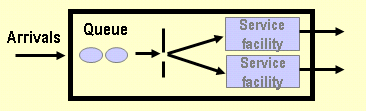
\includegraphics{/home/ivans/Workspace/ivans/penulisan-ilmiah/document/images/bab2/multi_channel_single_phase}\caption{Multi Channel \textendash{} Single Phase }
\end{figure}
 Sistem Multi Channel \textendash{} Single Phase terjadi di mana ada
dua atau lebih fasilitas pelayanan dialiri oleh antrian tunggal. Contohnya
adalah antrian pada sebuah bank dengan beberapa teller, pembelian
tiket atau karcis yang dilayani oleh beberapa loket, pembayaran dengan
beberapa kasir, dan lain-lain. 
\item Multi Channel \textendash{} Multi Phase 

\begin{figure}[H]
\centering{}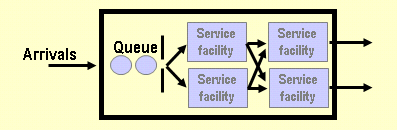
\includegraphics{/home/ivans/Workspace/ivans/penulisan-ilmiah/document/images/bab2/multi_channel_multi_phase}\caption{Multi Channel \textendash{} Multi Phase }
\end{figure}
 Sistem Multi Channel \textendash{} Multi Phase ini menunjukkan bahwa
setiap sistem mempunyai beberapa fasilitas pelayanan pada setiap tahap
sehingga terdapat lebih dari satu pelanggan yang dapat dilayani pada
waktu bersamaan. Contoh pada model ini adalah : pada pelayanan yang
dibarikan kepada pasien di rumah sakit dimulai dari pendaftarran,
diagnose, tindakan medis, samppai pembayaran, registrasi ulang mahasiswa
baru pada sebuah universitas, dan lain-lain. 
\end{enumerate}

\section{Web Server}

Web server adalah sebuah software yang memberikan layanan berbasis
data dan berfungsi menerima permintaan dari HTTP atau HTTPS pada klien
yang dikenal dan biasanya kita kenal dengan nama web browser dan untuk
mengirimkan kembali yang hasilnya dalam bentuk beberapa halaman web
dan pada umumnya akan berbentuk dokumen HTML. itulah pengertian web
server sebenarnya. dalam bentuk sederhana web server akan mengirim
data HTML kepada permintaan web Browser sehingga akan terlihat seperti
pada umumnya yaitu sebuah tampilan website.

\section{Aplikasi Web}

Dalam rekayasa perangkat lunak, suatu aplikasi web (bahasa Inggris:
web application atau sering disingkat webapp) adalah suatu aplikasi
yang diakses menggunakan penjelajah web melalui suatu jaringan seperti
Internet atau intranet. Ia juga merupakan suatu aplikasi perangkat
lunak komputer yang dikodekan dalam bahasa yang didukung penjelajah
web (seperti HTML, JavaScript, AJAX, Java, dll) dan bergantung pada
penjelajah tersebut untuk menampilkan aplikasi.

Aplikasi web menjadi populer karena kemudahan tersedianya aplikasi
klien untuk mengaksesnya, penjelajah web, yang kadang disebut sebagai
suatu thin client (klien tipis). Kemampuan untuk memperbarui dan memelihara
aplikasi web tanpa harus mendistribusikan dan menginstalasi perangkat
lunak pada kemungkinan ribuan komputer klien merupakan alasan kunci
popularitasnya. Aplikasi web yang umum misalnya webmail, toko ritel
daring, lelang daring, wiki, papan diskusi, weblog, serta MMORPG.

\section{AngularJS}

AngularJS merupakan framework javascript open source yang dirilis
oleh google pada tahun 2009. Konsep dari AngularJS adalah meningkatkan
fungsi dari HTML untuk membangun wepapp. Bayangkan awalnya HTML hanya
digunakan untuk membuat halaman website statis dan kini bisa berfungsi
untuk membuat wepapp dengan menggunakan AngularJS.\cite{key-3}.

\section{Java}

Java adalah nama sebuah bahasa pemrograman yang sangat terkenal. Sebagai
bahasa pemrograman, Java dapat digunakan untuk menulis program. Sebagaimana
diketahui, program adalah kumpulan instruksi yang ditujukan unutk
komputer. Melalui program, komputer dapat diatur agar melaksanakan
tugas tertentu sesuai yang ditentukan oleh pemrogram (orang yang membuat
program).\cite{key-2}.

\section{Mysql Server}

MySQL adalah sebuah perangkat lunak sistem manajemen basis data SQL
(bahasa Inggris: database management system) atau DBMS yang multithread,
multi-user, dengan sekitar 6 juta instalasi di seluruh dunia. MySQL
AB membuat MySQL tersedia sebagai perangkat lunak gratis dibawah lisensi
GNU General Public License (GPL), tetapi mereka juga menjual dibawah
lisensi komersial untuk kasus-kasus di mana penggunaannya tidak cocok
dengan penggunaan GPL.

\chapter{Analisa Dan Perancangan}

Pada bab ini dilakukan analisis dan perancangan berdasarkan teori
yang telah dijelaskan pada bab sebelumnya. Analisis dimulai dari masalah
membangun aplikasi ini menggunakan bahasa pemprograman java. Proses
pembuatan aplikasi ini melalui beberapa tahapan, mulai dari proses
analisa, profil pengguna, pembuatan struktur navigasi, perancangan
tampilan, pengujian dan langkah-langkah pembuatan aplikasi.

\section{Analisis}

Pada pembuatan aplikasi, diperlukan pembuatan analisa sistem. Analisa
sistem adalah penguraian dari suatu sistem yang utuh kedalam bagian-bagian
komponennya dengan maksud untuk mengidentifikasi dan mengevaluasi
permasalahan.

Mengidentifikasi (mengenal) masalah merupakan langkah pertama yang
dilakukan dalam tahap analisis sistem. Masalah dapat didefinisikan
sebagai suatu pertanyaan yang ingin dipecahkan.

Sama halnya dalam pembuatan aplikasi ini. Penulis memilih informasi
mengenai antrian di suatu rumah sakit swasta untuk mempermudah pihak
rumah sakit dalam melayani pasien yang mendaftar.

Selanjutnya, analisis masalah dapat dilakukan. Pada bagian analisis,
terdiri dari atas analisis fungsional dan analisis permasalahan \textit{resource}.

\subsection{Analisis Fungsional}

Analisis fungsional merupakan paparan mengenai fitur-fitur yang akan
dimasukkan kedalam aplikasi ini. Fitur-fitur tersebut antara lain
pengaturan jadwal dokter, pendaftaran tiket antrian, print tiket,
pemanggilan suara berdasarkan nomor tiket, history pasien dan pembelian
obat.

\subsection{Analisis Permasalahan Resource (Sumber Daya)}

Dikarnakan aplikasi yang akan di buat adalah webapp dengan menggunakan
full javascript pada bagian interface, maka untuk mempercepat load
resource sangat di perlukan penempatan file javascript di akhir file
index, dan meminimkan pemakaian gambar.

\section{Struktur Navigasi}

Struktur navigasi adalah urutan alur informasi dari suatu aplikasi
multimedia. Dengan menggunakan struktur navigasi yang tepat maka suatu
aplikasi mempunyai suatu pedoman dan arah informasi yang jelas. Dalam
proses pembuatan aplikasi ini penulis menggunakan struktur navigasi
hirarki. Karena dalam beberapa menu terdapat percabangan atau sub
menu pada menu utama.

\subsection{Struktur Navigasi Admin}

\begin{figure}[H]
\centering{}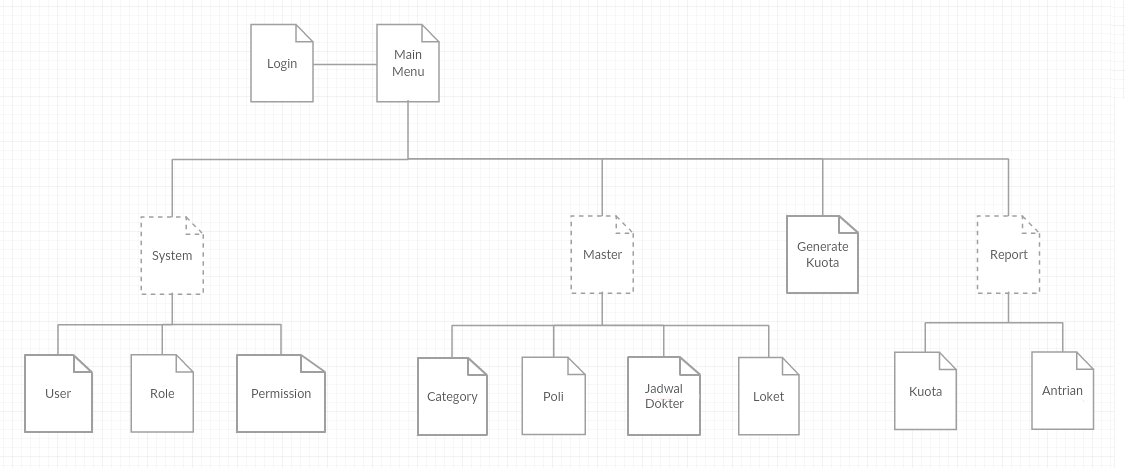
\includegraphics[width=0.65\paperwidth]{/home/ivans/Workspace/ivans/penulisan-ilmiah/document/images/struktur_navigasi/struktur_navigasi_admin}\caption{Struktur Navigasi Admin}
\end{figure}
 

\subsection{Struktur Navigasi Loket}

\begin{figure}[H]
\centering{}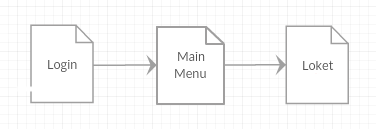
\includegraphics[width=0.4\paperwidth]{/home/ivans/Workspace/ivans/penulisan-ilmiah/document/images/struktur_navigasi/struktur_navigasi_loket}\caption{Struktur Navigasi Loket}
\end{figure}
 

\subsection{Struktur Navigasi Information Monitor}

\begin{figure}[H]
\centering{}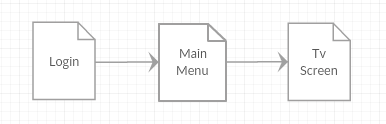
\includegraphics[width=0.4\paperwidth]{/home/ivans/Workspace/ivans/penulisan-ilmiah/document/images/struktur_navigasi/struktur_navigasi_tv}\caption{Struktur Navigasi Admin}
\end{figure}
 

\subsection{Struktur Navigasi Pendaftaran Antrian}

\begin{figure}[H]
\centering{}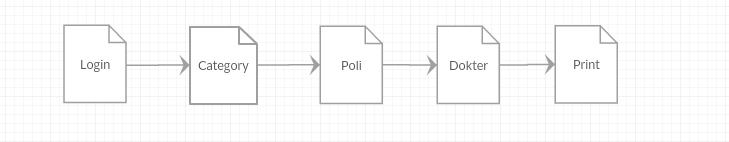
\includegraphics[width=0.6\paperwidth]{/home/ivans/Workspace/ivans/penulisan-ilmiah/document/images/struktur_navigasi/struktur_navigasi_pendaftaran}\caption{Struktur Navigasi Admin}
\end{figure}

\newpage{}

\section{Rancangan Tampilan}

Rancangan tampilan aplikasi merupakan hal yang sangat penting untuk
kemudahan para pengguna saat berinteraksi dengan sebuah aplikasi dan
kemudahan mendapatkan informasi yang dibutuhkan dengan cepat dan efisien.

Dengan memberikan deskripsi ini, penulis berharap sebelum tahap penjelasan
proses pembuatan, aplikasi ini sudah dapat dipandang secara utuh dengan
kata lain dapat dipahami secara jelas apa yang akan dibahas pada proses
pembuatan aplikasi ini.

\subsection{Rancangan Halaman Login}

\begin{figure}[H]
\centering{}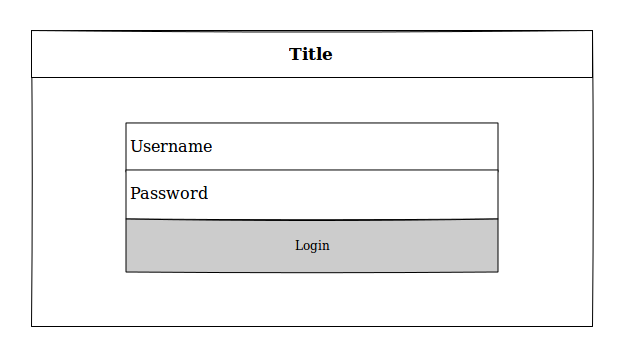
\includegraphics[width=0.65\paperwidth]{/home/ivans/Workspace/ivans/penulisan-ilmiah/document/images/rancangan/rancangan_login}\caption{Rancangan Login}
\end{figure}
 Pada rancangan halaman login terdapat 2 textfield yaitu untuk input
username dan password.

\subsection{Rancangan Halaman System dan Master.}

\begin{figure}[H]
\centering{}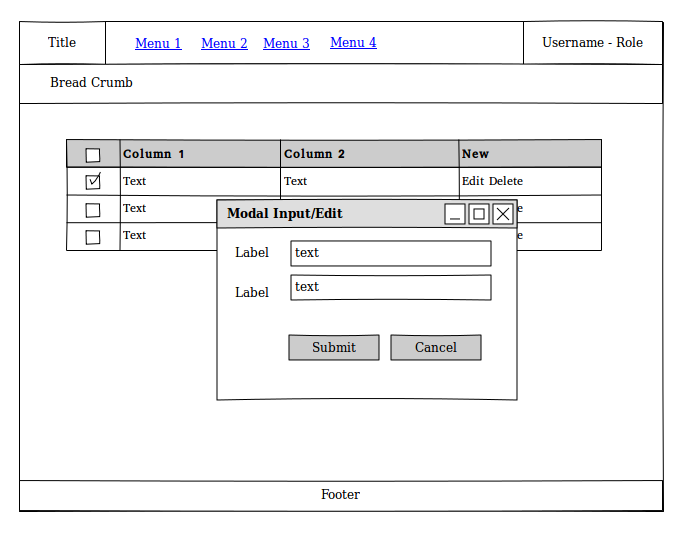
\includegraphics[width=0.65\paperwidth]{/home/ivans/Workspace/ivans/penulisan-ilmiah/document/images/rancangan/rancangan_master}\caption{Rancangan Halaman System Dan Master}
\end{figure}
 Pada rancangan halaman master dan system terdapat proses CRUD (Create,
Read, Update dan Delete), dimana yang di tampilkan pada halaman hanya
list/table nya saja, untuk form input/update dibuatkan modal yang
akan terbuka jika button input/edit di klik.

\subsection{Rancangan Halaman Loket}

\begin{figure}[H]
\centering{}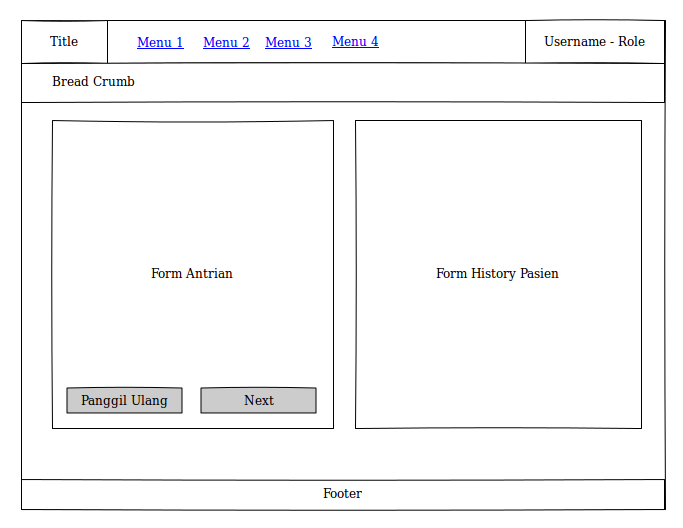
\includegraphics[width=0.65\paperwidth]{/home/ivans/Workspace/ivans/penulisan-ilmiah/document/images/rancangan/rancangan_loket}\caption{Rancangan Halaman Loket}
\end{figure}
 Pada rancangan halaman loket terdapat 2 panel utama, panel pertama/form
antrian digunakan untuk menampilkan informasi antrian seperti no antrian
sekarang, no antrian berikutnya, button pemanggilan dan button panggil
ulang. Sedangkan panel kedua/form history pasien digunakan untuk mendaftarkan
pasien dan menambahkan history pendaftaran pasien.

\subsection{Rancangan Halaman Information Monitor}

\begin{figure}[H]
\centering{}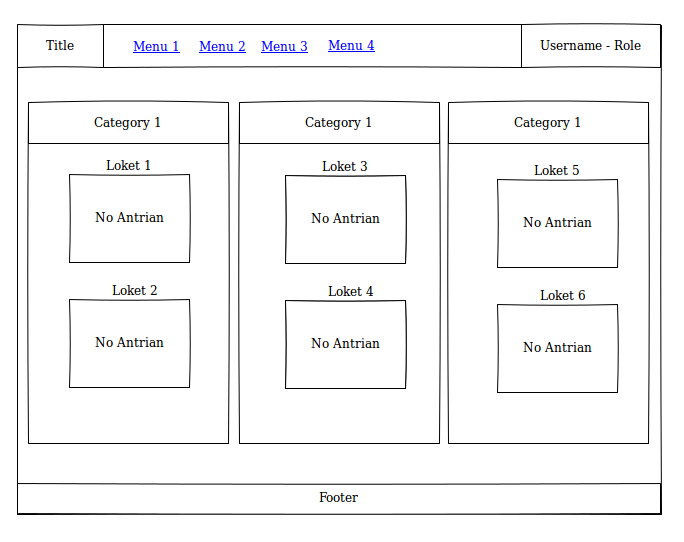
\includegraphics[width=0.65\paperwidth]{/home/ivans/Workspace/ivans/penulisan-ilmiah/document/images/rancangan/rancangan_monitor}\caption{Rancangan Halaman Screen Information}
\end{figure}
 Pada rancangan halaman ini digunakan untuk menampilkan no antrian
yang sedang di proses oleh masing masing loket, dengan urutan kategori-loket-nomor.

\subsection{Rancangan Halaman Pendaftaran}

\begin{figure}[H]
\centering{}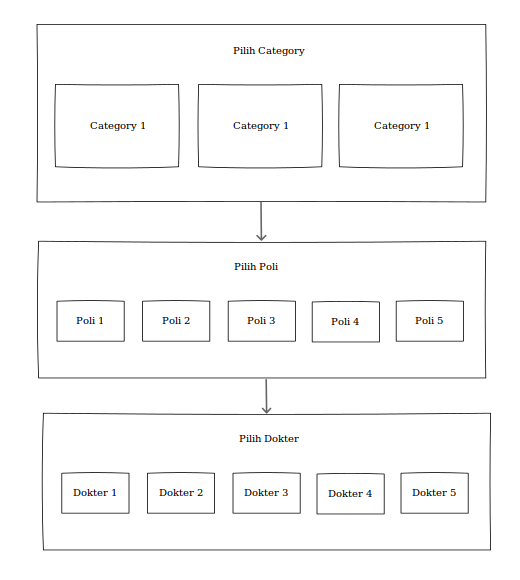
\includegraphics[width=0.65\paperwidth]{/home/ivans/Workspace/ivans/penulisan-ilmiah/document/images/rancangan/rancangan_pendaftaran}\caption{Rancangan Halaman Pendaftaran}
\end{figure}
 Pada rancangan halaman pendaftaran terdapat 3 form dinamis, yang
pertama form kategori, setelah kategori dipilih akan muncul form poli
sesuai dengan kategori yang dipilih, dan form terakhir yaitu form
untuk memilih dokter yang tersedia dengan poli yang sudah di pilih 

\subsection{Rancangan Report}

\begin{figure}[H]
\centering{}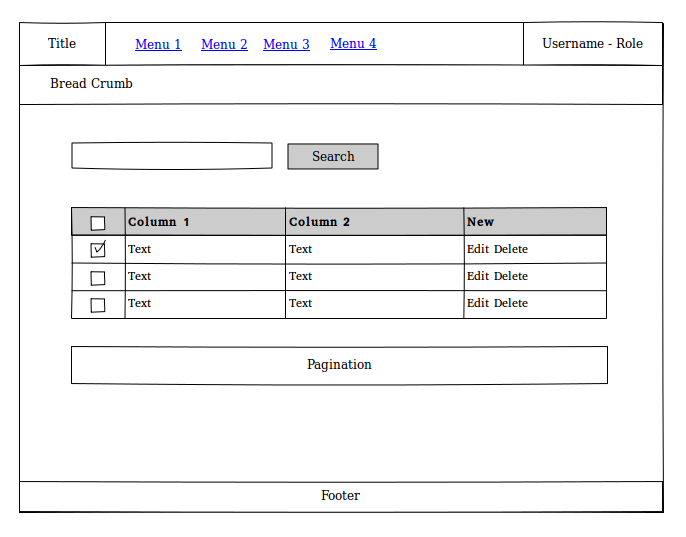
\includegraphics[width=0.65\paperwidth]{/home/ivans/Workspace/ivans/penulisan-ilmiah/document/images/rancangan/rancangan_report}\caption{Rancangan Halaman Report}
\end{figure}
 Pada rancangan halaman report terdapat 3 komponen utama yaitu 
\begin{enumerate}
\item Filter/Form search untuk memudahkan user mencari data.
\item Table/List untuk menampilkan data.
\item Pagination 
\end{enumerate}

\section{Implementasi Aplikasi}

Pada pembuatan aplikasi sistem antrian rumah sakit berbasis web ini
penulis menggunakan sistem operasi Linux Ubuntu 16.04 dengan Java
versi \textquotedbl{}1.8.0\_91\textquotedbl{}.

\subsection{Instalasi Java Runtime Environment (JRE) dan Java Development Kit
(JDK)}

Java Runtime Environment dan Java Development Kit harus sudah terinstall
karena aplikasi yang akan dibuat menggunakan pemprograman java. Langkah-langkah
installasinya adalah :
\begin{enumerate}
\item Download JDK di http://www.oracle.com/ 
\item Extract file JDK yang sudah di download
\item Open terminal
\item Open file /etc/profile dengan perintah ``\$ sudo nano /etc/profile''
\item Export JDK pada /etc/profile dengan menambahkan : ``export PATH=\$PATH:/lokasi\_jdk/bin''
\item Restart, dan untuk mengetahui apakah java sudah terinstall dengan
perintah ``\$ java -version''
\end{enumerate}

\subsection{Instalasi Maven}

Maven harus sudah terinstall karena aplikasi akan di jalankan menggunakan
aplikasi ini. Langkah-langkah installasinya adalah :
\begin{enumerate}
\item Open terminal
\item Install Mysql dengan perintah ``\$ sudo apt-get install maven''
\item Restart, dan untuk mengetahui apakah maven sudah terinstall dengan
perintah ``\$ mvn -version''
\end{enumerate}

\subsection{Instalasi Mysql}

Sebelum aplikasi ini berjalan DBMS Mysql harus sudah terinstall, Langkah-langkah
installasinya :
\begin{enumerate}
\item Open terminal
\item Install Mysql dengan perintah ``\$ sudo apt-get install mysql-server-5.6''
\item Setelah instalasi selesai, open Mysql dengan perintah ``\$ mysql
-uroot -p''
\item Buat database baru untuk penyimpanan data antrian dengan perintah
``create database antrian\_development''
\end{enumerate}

\subsection{Implementasi Webapp}

Berikutnya penulis akan menampilkan desain dari tampilan webapp sistem
antrian ini. Untuk lebih jelas nya berikut ini adalah beberapa tampilan
nya:
\begin{enumerate}
\item Halaman Login 

\begin{figure}[H]
\centering{}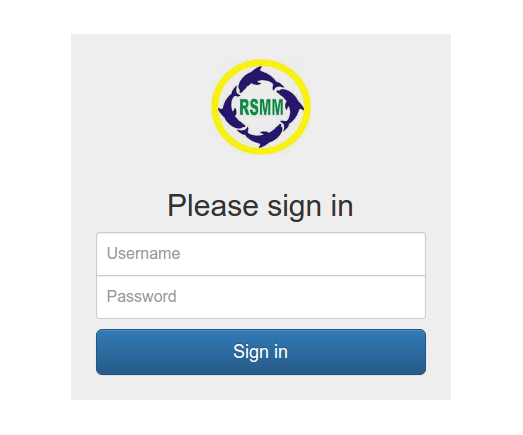
\includegraphics[width=0.5\paperwidth]{/home/ivans/Workspace/ivans/penulisan-ilmiah/document/images/screenshot/login}\caption{Halaman Login }
\end{figure}
 Sebelum masuk kedalam web utama, user akan login melalui halaman
ini. Dalam halaman ini hanya terdapat field username dan password
yang harus di isi untuk divalidasi apakah sudah benar dengan data
yang ada di database.
\item Halaman Permission 

\begin{figure}[H]
\centering{}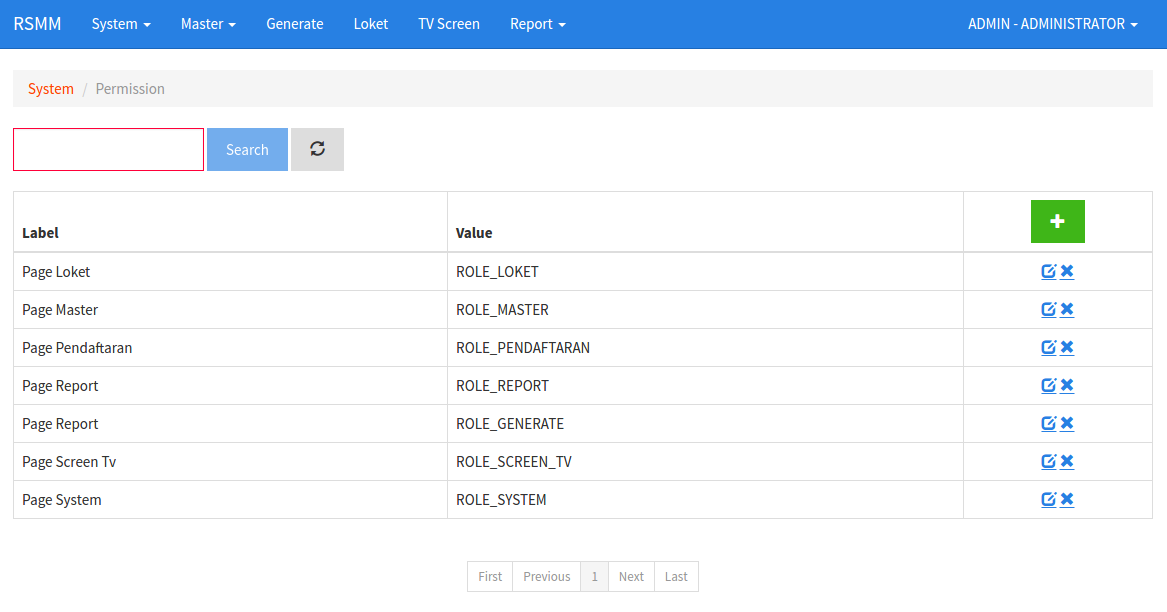
\includegraphics[width=0.65\paperwidth]{/home/ivans/Workspace/ivans/penulisan-ilmiah/document/images/screenshot/permission}\caption{Halaman Permission }
\end{figure}
 Pada halaman ini digunakan oleh admin untuk mempermudah dalam mengatur
permission yang akan di gunakan aplikasi. Pada list yang ditampilkan
terdapat \textbf{label} sebagai penamaan dan \textbf{value} sebagai
nilai yang digunakan oleh aplikasi dalam menentukan permission aplikasi. 
\item Halaman Role 

\begin{figure}[H]
\centering{}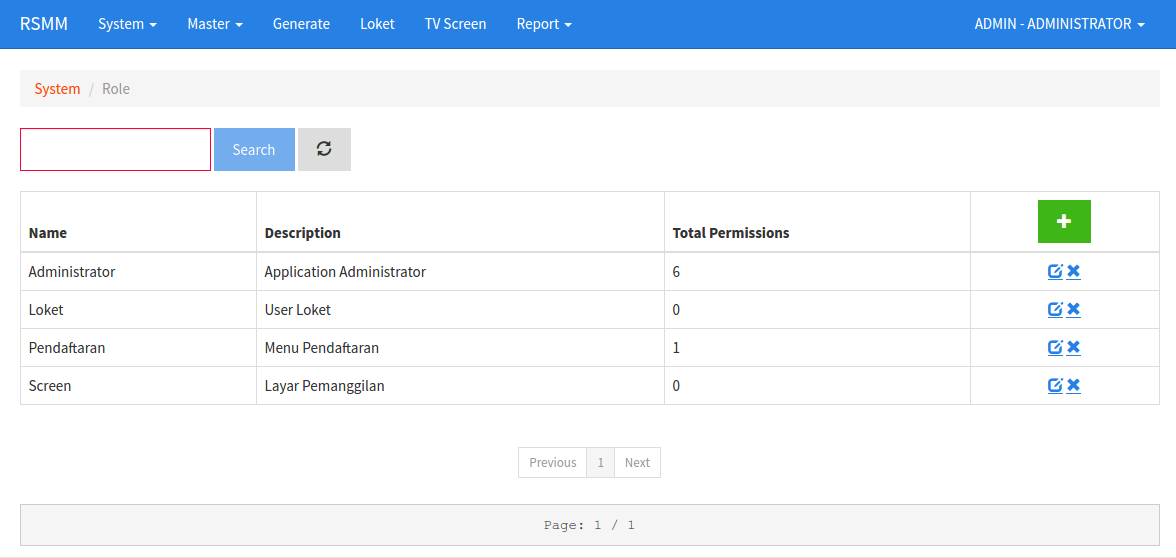
\includegraphics[width=0.65\paperwidth]{/home/ivans/Workspace/ivans/penulisan-ilmiah/document/images/screenshot/role}\caption{Halaman Role }
\end{figure}
Pada halaman ini digunakan oleh admin untuk membuat role dan menambahkan
hak akses/permission yang boleh digunakan oleh user dengan role tersebut.
Pada list yang ditampilkan terdapat \textbf{name} sebagai nama role,
\textbf{description} sebagai keterangan tambahan dan \textbf{total
permissions }yaitu total permission yang di miliki role tersebut.
\item Halaman User 

\begin{figure}[H]
\centering{}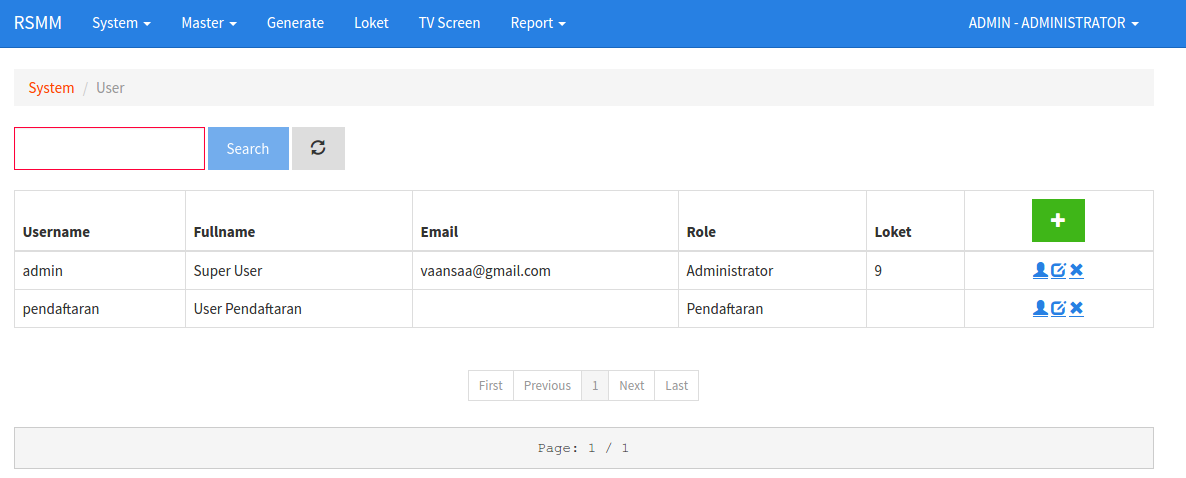
\includegraphics[width=0.65\paperwidth]{/home/ivans/Workspace/ivans/penulisan-ilmiah/document/images/screenshot/user}\caption{Halaman User }
\end{figure}
Pada halaman ini digunakan oleh admin untuk managemen user. Pada list
yang ditampilkan terdapat \textbf{username}, \textbf{fullname}, \textbf{email},
\textbf{role} dan \textbf{loket}.
\item Halaman Master Kategori 

\begin{figure}[H]
\centering{}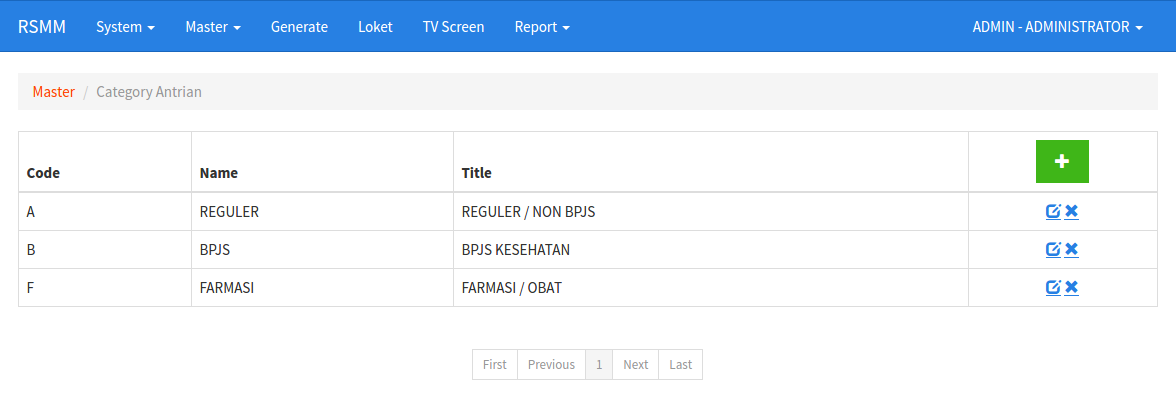
\includegraphics[width=0.65\paperwidth]{/home/ivans/Workspace/ivans/penulisan-ilmiah/document/images/screenshot/kategory}\caption{Halaman Master Kategori }
\end{figure}
Pada halaman ini digunakan oleh admin untuk managemen kategori loket.
Pada list yang ditampilkan terdapat \textbf{code}, \textbf{name} dan
\textbf{title.}
\item Halaman Master Poli 

\begin{figure}[H]
\centering{}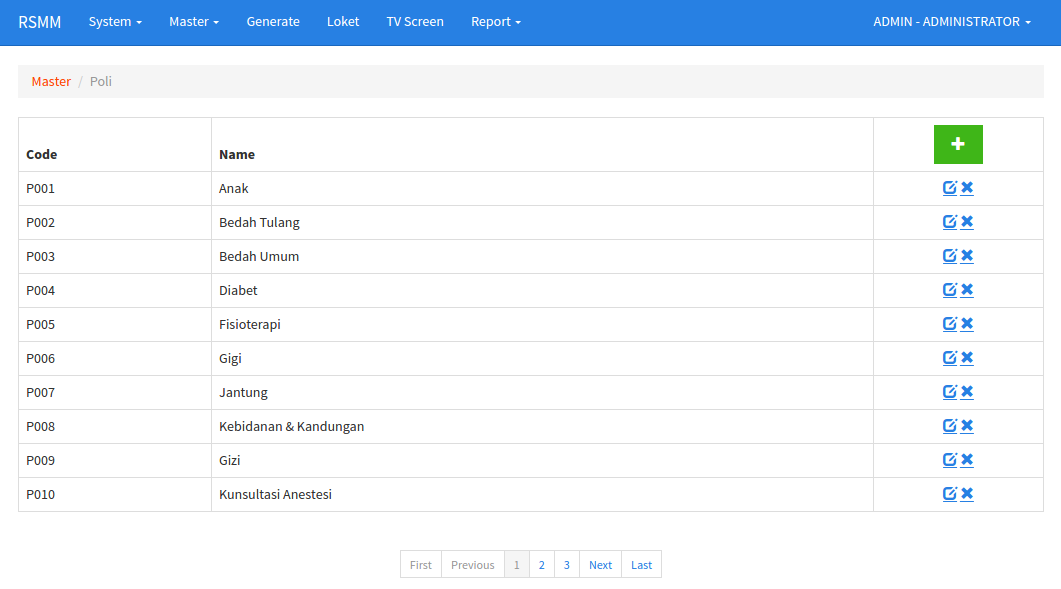
\includegraphics[width=0.65\paperwidth]{/home/ivans/Workspace/ivans/penulisan-ilmiah/document/images/screenshot/poli}\caption{Halaman Master Poli }
\end{figure}
Pada halaman ini digunakan oleh admin untuk managemen poli. Pada list
yang ditampilkan terdapat \textbf{code }dan \textbf{name}.
\item Halaman Master Dokter 

\begin{figure}[H]
\centering{}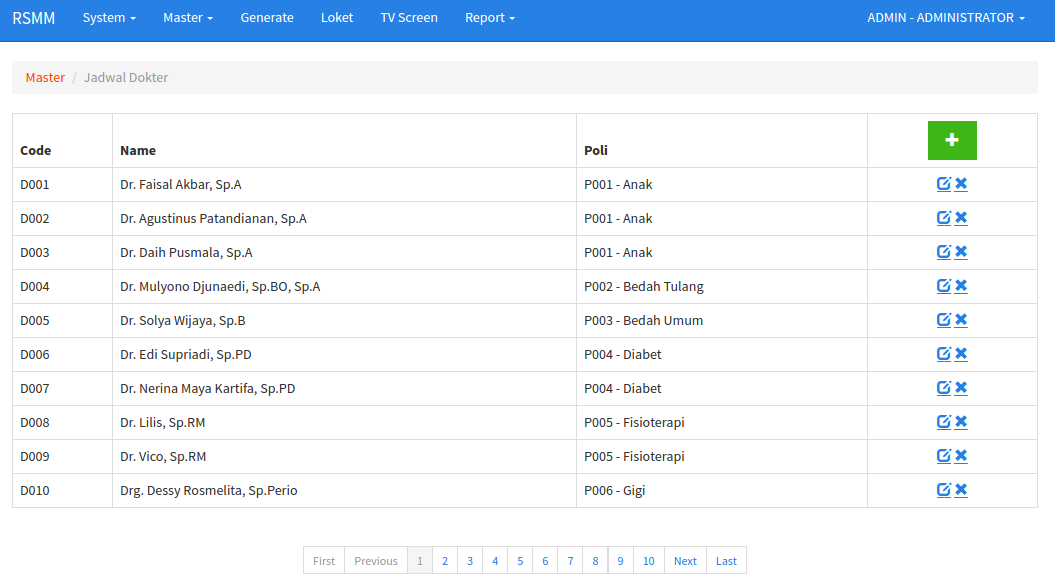
\includegraphics[width=0.65\paperwidth]{/home/ivans/Workspace/ivans/penulisan-ilmiah/document/images/screenshot/dokter}\caption{Halaman Master Dokter }
\end{figure}
Pada halaman ini digunakan oleh admin untuk managemen dokter, mengatur
jadwal praktek dan kuota pasien. Pada list yang ditampilkan terdapat
\textbf{code}, \textbf{name} dan\textbf{ poli}.
\item Halaman Master Loket 

\begin{figure}[H]
\centering{}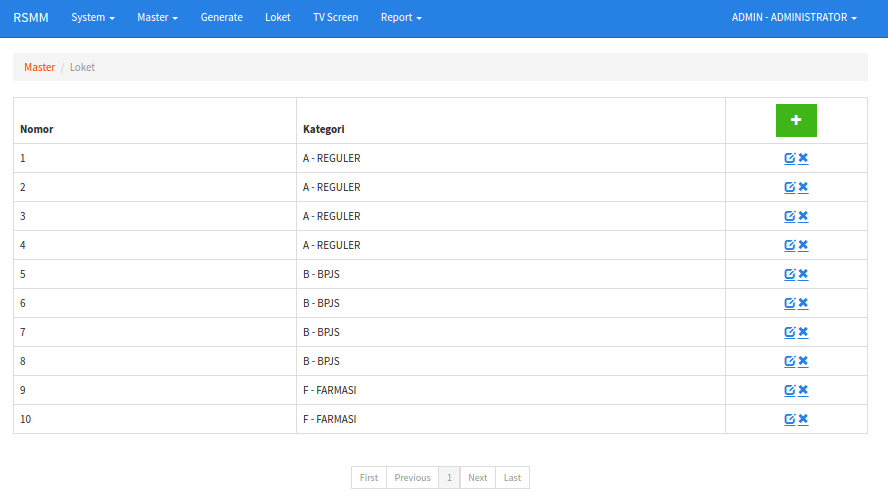
\includegraphics[width=0.65\paperwidth]{/home/ivans/Workspace/ivans/penulisan-ilmiah/document/images/screenshot/loket}\caption{Halaman Master Loket }
\end{figure}
Pada halaman ini digunakan oleh admin untuk managemen nomor loket
dan jenis kategori loket tersebut. Pada list yang ditampilkan terdapat
\textbf{nomor} dan \textbf{kategori}.
\item Halaman Generate Kuota Harian

\begin{figure}[H]
\centering{}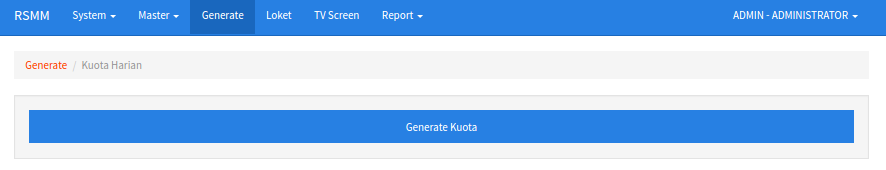
\includegraphics[width=0.65\paperwidth]{/home/ivans/Workspace/ivans/penulisan-ilmiah/document/images/screenshot/generate}\caption{Halaman Generate Kuota }
\end{figure}
Pada halaman ini hanya ada 1 button yaitu \textbf{generate kuota}
yang digunakan admin untuk generate data kuota. Data ini digunakan
sebagai penanda apakah loket libur atau tidak, data kuota di ambil
dari master dokter.
\item Halaman Report Kuota

\begin{figure}[H]
\centering{}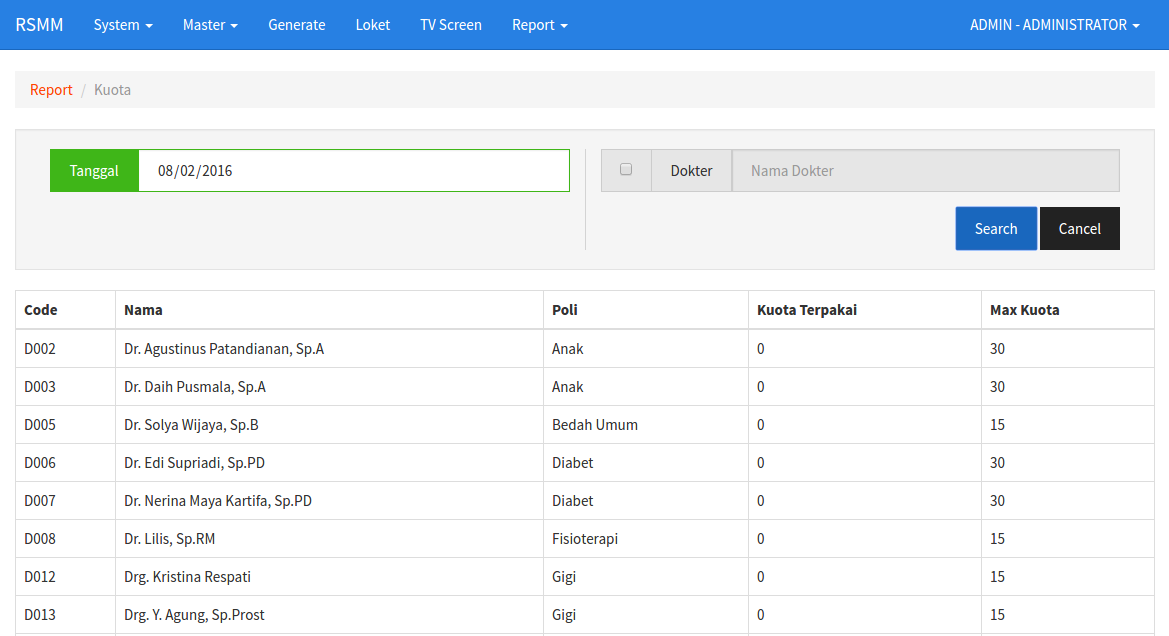
\includegraphics[width=0.65\paperwidth]{/home/ivans/Workspace/ivans/penulisan-ilmiah/document/images/screenshot/report_kuota}\caption{Halaman Report Kuota }
\end{figure}
Pada halaman report ini menampilkan maximum dan jumlah kuota yang
telah digunakan pada setiap dokter, pada report tersebut terdapat
2 filter yaitu berdasarkan tanggal dan dokter.
\item Halaman Report Antian

\begin{figure}[H]
\centering{}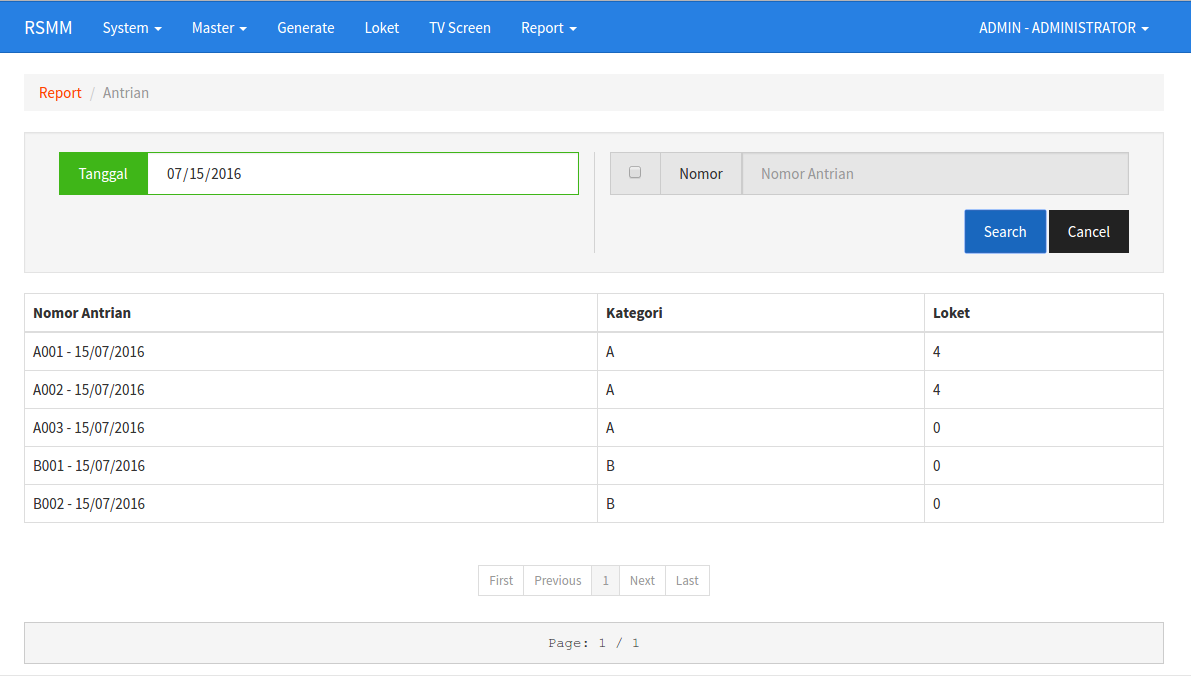
\includegraphics[width=0.65\paperwidth]{/home/ivans/Workspace/ivans/penulisan-ilmiah/document/images/screenshot/report_antrian}\caption{Halaman Report Antrian }
\end{figure}
Pada halaman report ini menampilkan data pendaftar nomor antiran,
pada report tersebut terdapat 2 filter yaitu berdasarkan tanggal dan
nomor antrian.
\item Halaman Loket

\begin{figure}[H]
\centering{}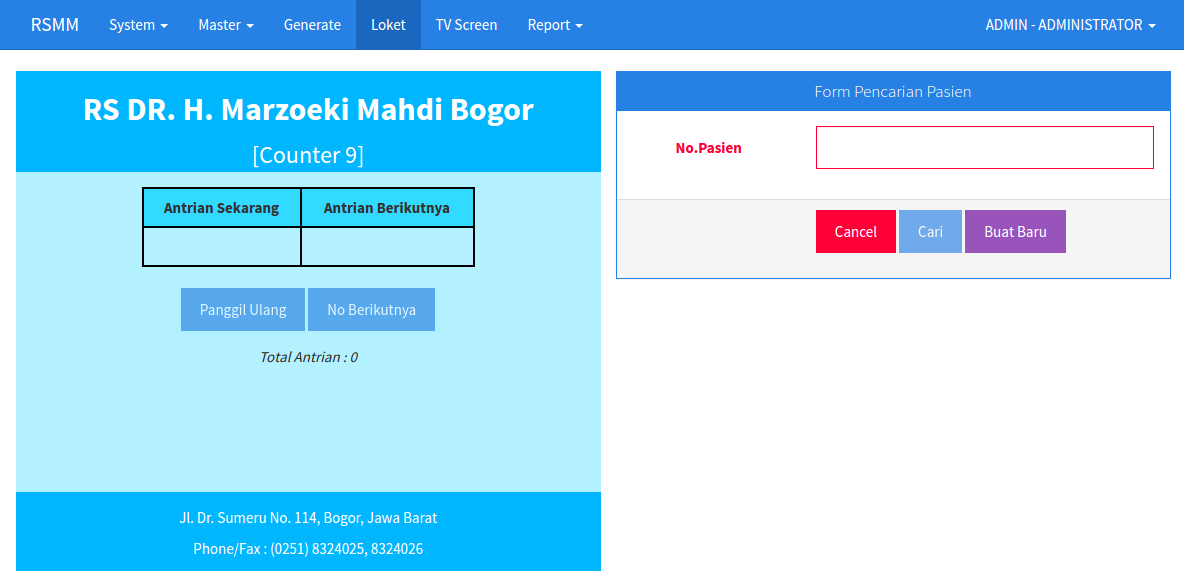
\includegraphics[width=0.65\paperwidth]{/home/ivans/Workspace/ivans/penulisan-ilmiah/document/images/screenshot/loket_page}\caption{Halaman Loket}
\end{figure}
Halaman loket ini merupakan halaman transaksi utama. Pada bagian kiri
terdapat form antian yang digunakan untuk menampilkan nomor antian
yang sedang di proses, nomor antrian berikutnya dan total antrian.
Dan bagian kanan merupakan form yang digunakan untuk menyimpan dan
mencari history pasien tersebut. 
\item Halaman Information Monitor

\begin{figure}[H]
\centering{}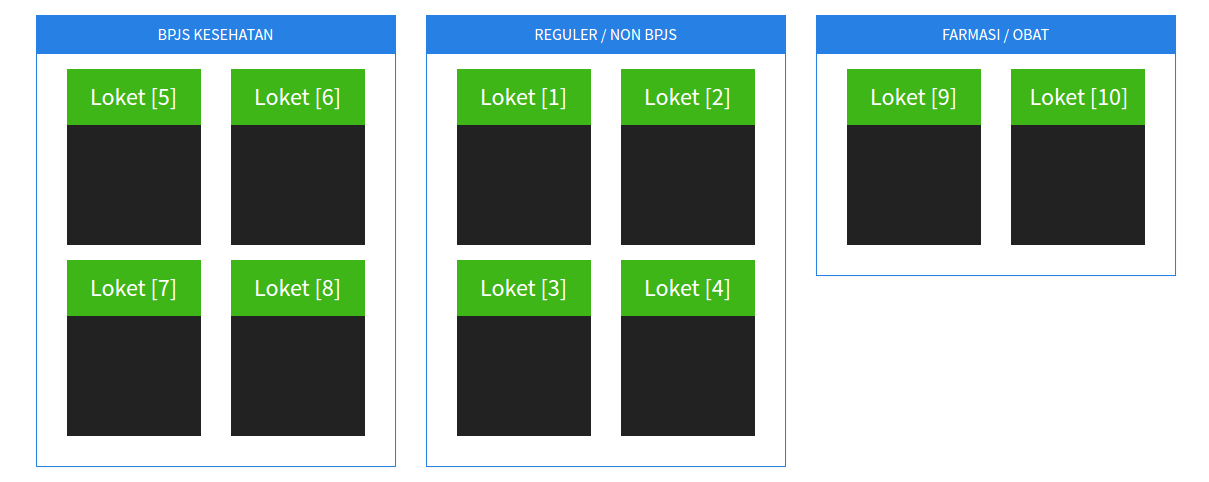
\includegraphics[width=0.65\paperwidth]{/home/ivans/Workspace/ivans/penulisan-ilmiah/document/images/screenshot/screen}\caption{Halaman Information Monitor }
\end{figure}
Halaman ini digunakan untuk menampilkan informasi tentang nomor antrian
yang sedang di proses pada setiap loket, pada box biru merupakan kategori
loket yang berisi loket-loket yang merupakan bagian dari kategori
tersebut.
\item Halaman Pendaftaran

\begin{figure}[H]
\centering{}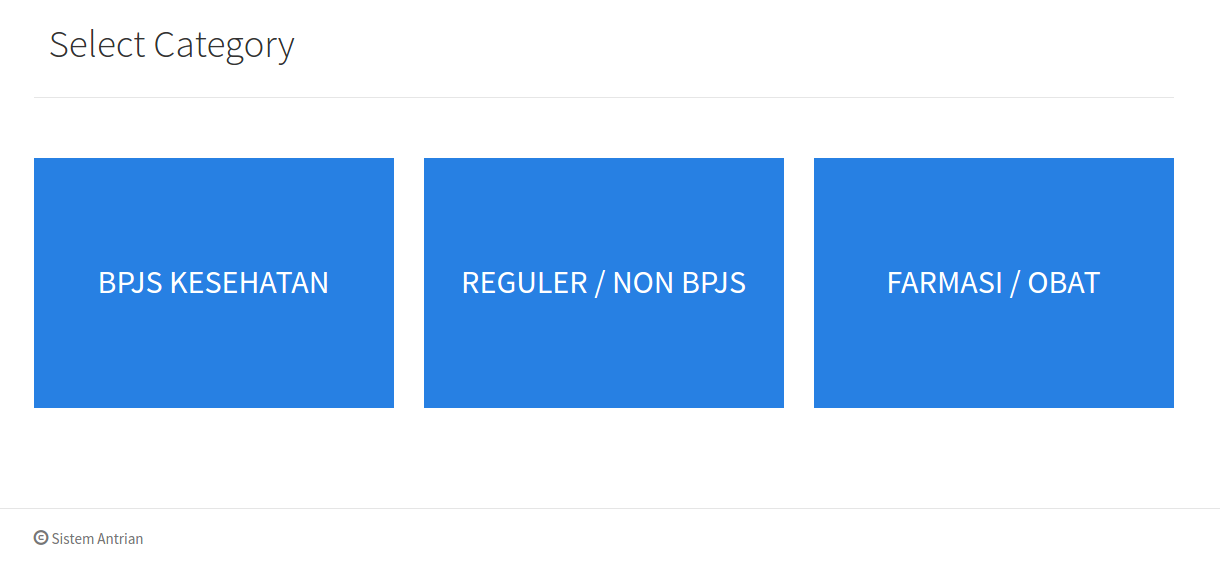
\includegraphics[width=0.65\paperwidth]{/home/ivans/Workspace/ivans/penulisan-ilmiah/document/images/screenshot/select_category}\caption{Halaman Pemilihan Kategori }
\end{figure}
Halaman awal pendaftaaran terdapat button - button yang merupakan
kategori loket yang ingin di pilih.
\begin{figure}[H]
\centering{}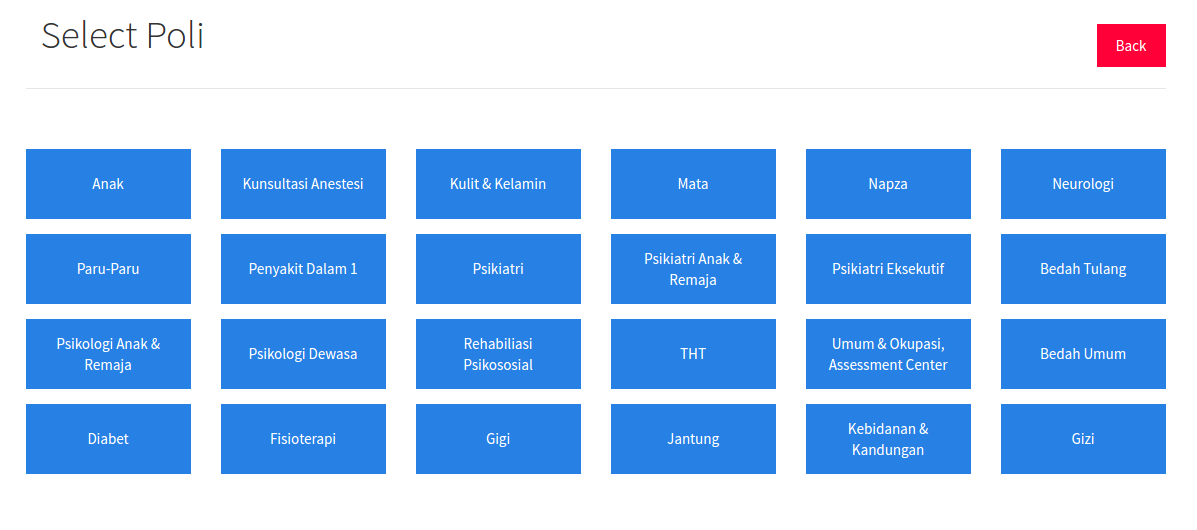
\includegraphics[width=0.65\paperwidth]{/home/ivans/Workspace/ivans/penulisan-ilmiah/document/images/screenshot/select_poli}\caption{Halaman Pemilihan Poli }
\end{figure}
Setelah memilih kategori user akan berpindah form dengan button -
button yang merupakan poli yang ingin di pilih.
\begin{figure}[H]
\centering{}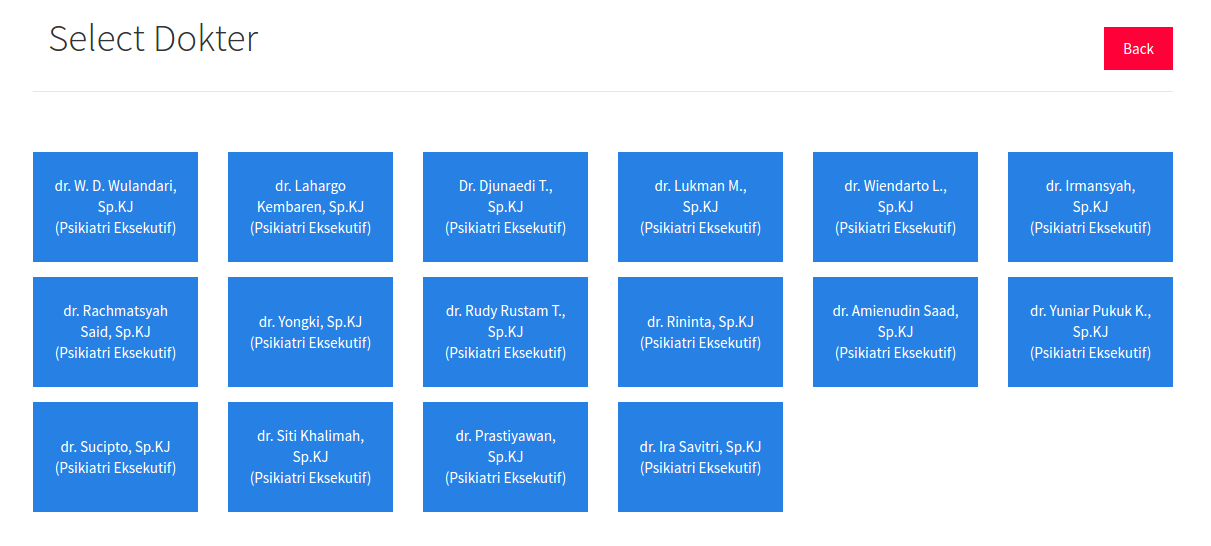
\includegraphics[width=0.65\paperwidth]{/home/ivans/Workspace/ivans/penulisan-ilmiah/document/images/screenshot/select_dokter}\caption{Halaman Pemilihan dokter }
\end{figure}
Setelah memilih poli user akan berpindah form dengan button - button
yang merupakan dokter yang ingin di pilih.
\begin{figure}[H]
\centering{}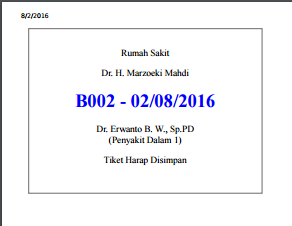
\includegraphics[width=0.4\paperwidth]{/home/ivans/Workspace/ivans/penulisan-ilmiah/document/images/screenshot/print}\caption{Tiket Pendaftaran}
\end{figure}
Setelah memilih dokter makan user akan langsung mencetak tiket pendaftaran
loket
\end{enumerate}
\begin{thebibliography}{1}
\bibitem{key-1}Djati, Bonett SL . \textit{Simulasi Teori dan Aplikasinya}.
Andi Publisher. Yogyakarta:2007.

\begin{flushleft}
\bibitem[2]{key-2}Kodir, Abdul. \textit{Buku Pertama Belajar Pemrograman
Java Untuk Pemula}. Mediakom. Yogyakarta:2013. 

\par\end{flushleft}\begin{flushleft}
\bibitem[3]{key-3}Febrian, Rully. (2014, Agustus). Apa Itu AngularJS.
Retrieved from http://www.dumetschool.com/

\par\end{flushleft}\bibitem[4]{key-4}Kakiay, Thomas J. Dasar Teori Antrian Untuk Kehidupan
Nyata. Andi Offset. Yogyakarta:2004
\end{thebibliography}

\end{document}
